\chapter{Analyzing Series and Parallel Circuits}
\label{chSeriesParallel}

% FIXME - do I define "voltage drop" anywhere?
% FIXME - make sure I mention that current in a series circuit is the same for the whole series
% FIXME - be sure I define subcircuit somewhere in this chapter


In the Chapter~\ref{chapFirstCircuit} we looked at our very first circuit and how to draw it using a circuit diagram.
In this chapter, we are going to look at different ways components can be hooked together and what they mean for your circuit.

\section{Series Circuits}

The circuit built in Chapter~\ref{chapFirstCircuit} is considered a \glossterm{series circuit} because all of the components are connected end-to-end, one after another.
In a series circuit, there is only one pathway for the current to flow, making analyzing the circuit fairly simple.

It does not matter how \emph{many} components are connected together---as long as all of the components are connected one after another, the circuit is considered a series circuit.
Figure~\ref{figSeriesComponents} shows a series circuit with several components included.

\simplegraphicsfigure{A Series Circuit with Several Components}{SeriesComponents}{0.08}

If all of the components are in a series, then even if there are multiple resistors scattered throughout the circuit, you can figure out the total resistance of the circuit just by adding together all of the resistances.
This is known as the \glossterm{equivalent resistance} of the series.

In this example, if R1 is 100\si{\ohm}, R2 is 350\si{\ohm}, and R3 is 225\si{\ohm}, then the total series resistance of the circuit will be $100 + 350 + 225 = 675\,\si{\ohm}$.

That means that the current is easy to figure out as well.
If we ignore the LEDs (since we have not yet learned to calculate using them), then we can use the total series resistance to calculate current the same way we did with the single resistor.

Since the voltage is 9 volts, then we can use Ohm's law to find out the current going through the system.

$$I = V / R = 9 / 675 = 0.013\,\si{\ampere}$$

Note that \si{\ampere} stands for ampere, and we will be using this in our calculations from here on out.
However, in electronics, we usually measure in milliamps (abbreviated as \si{\milli\ampere}), so let us convert:

$$ 0.013 * 1000 = 13\,\si{\milli\ampere}$$

So, our circuit will draw about 13 milliamps of current.
This amount of current is the same amount running through all of the components in the series.

\section{Parallel Circuits}

Circuits are wired into a \glossterm{parallel circuit} if one or more of their components are arranged into multiple branches.

Figure~\ref{figSimpleParallel} shows a simple circuit with two resistors in parallel.
In this figure, the circuit has \emph{two} branches.
R1 is in the first branch, and R2 is in the second branch.
The place where the branch occurs is called a \glossterm{junction}, and is usually marked with a dot to show that all the wires there are connected.

\simplegraphicsfigure{Two Resistors Wired in Parallel}{SimpleParallel}{0.08}

In a parallel circuit, electricity will flow through both branches simultaneously.
Some of the current will go through R1 and some of it will go through R2.
This makes determining the total amount of current more difficult, as we have to take into account more than one branch.

However, there are two additional laws we can use to help us out, known as \glossterm{Kirchoff's circuit laws}.
The guy's name is hard to spell, but his rules are actually fairly easy to understand.

\subsection{Kirchoff's Current Law}

The first law is known as \glossterm{Kirchoff's current law}.
Kirchoff's current law states that, at any junction, the total amount of current going \emph{into} a junction is exactly the same as the total amount of current going \emph{out} of a junction.
This should make sense to us.
Think about traffic at a four-way intersection.
The same number of cars that enter that intersection must be the same number of cars that leave the intersection.
We can't create cars out of thin air, therefore each car leaving must have come in.
Cars don't magically disappear, therefore each car entering must leave at some point.
Therefore, Kirchoff's circuit law says that if you add up all of the traffic going in it will equal the amount going out.

\begin{advsidebar}{Another Way of Looking at It}
Another way to say this is that the total amount of all of the currents at a junction is zero.
That is, if we consider currents coming in to the junction to be positive and currents going out of the junction to be negative, then their total will be zero since the size of the currents coming in must equal the size of the currents going out.
\end{advsidebar}

So, let's look at a junction.
Figure~\ref{figSimpleJunction1} shows a junction where one wire is bringing current in, and it branches with two wires bringing current out.  
The first wire going out has $0.75\,\si{\ampere}$ of current, and the second wire going out has $0.34\,\si{\ampere}$ of current.
How much current is going into the junction from the left?

\simplegraphicsfigure{A Simple Junction}{SimpleJunction1}{0.08}

Since the total coming in must equal the total coming out, then that means the total coming in must be 

$$0.75\,\si{\ampere} + 0.34\,\si{\ampere} = 1.09\,\si{\ampere}$$

Therefore, the total amount of current coming into the circuit is $1.09\,\si{\ampere}$.

Now, lets say we had a junction of four wires.  
In the first wire, we have $0.23\,\si{\ampere}$ of current coming in.
On the second wire, we have $0.15\,\si{\ampere}$ of current going out.
On the third wire, we have $0.20\,\si{ampere}$ of current going out.
What must be happening on the fourth wire?
Is current coming in or going out on that wire?

To figure that out, we have to look at the totals so far.
Coming in, we have the one wire at $0.23\,\si{\ampere}$.
Going out, we have the two wires for a total of $0.15\,\si{\ampere} + 0.20\,\si{\ampere} = 0.35\,\si{\ampere}$.
Since we only have $0.23\,\myamp$ coming in, but there is $0.35\,\myamp$ going out, that means that the fourth wire must be bringing current in.
Therefore, the amount that this fourth wire must be bringing in is $0.35\,\myamp - 0.23\,\myamp = 0.12\,\myamp$.

\subsection{Kirchoff's Voltage Law}

Kirchoff's current law makes a lot of sense, because the amount of ``stuff'' coming in is the same as the amount of ``stuff'' going out.
This is similar to our everyday experience.
Kirchoff's voltage law, however, is a bit more tricky.
\glossterm{Kirchoff's voltage law} states that, given any two points on a circuit at a particular time, that no matter what path is travelled to get between those two points, the difference in voltage between the two points (known as the \glossterm{voltage drop}) is the same \emph{no matter what pathway you take to get there}.

Figures~\ref{figKirchoffVoltageLawExample0}~and~\ref{figKirchoffVoltageLawExampleComposite} illustrates this point.
If we wanted to measure the voltage drop between the two points indicated (A and B), then that voltage drop, at least at a particular point in time, will be the same no matter what pathway electricity travels.
The direct route between the two points has the same voltage drop as the more winding pathways, no matter what the values of the resistors are.

\simplegraphicsfigure{A Circuit With Many Parallel Paths}{KirchoffVoltageLawExample0}{0.08}
\simplegraphicsfigure{All Paths Between Two Points Have the Same Voltage Drop}{KirchoffVoltageLawExampleComposite}{0.05}

So how does that square with Ohm's law?

The way it works is that Ohm's law will cause all of the \emph{currents} through each part of the circuit to adjust in order to make sure that the \emph{voltage} stays the same.

As you can see, the voltage drop between A and B \emph{must} be 9 volts because the battery is a 9-volt battery, and there are no components (only wires) between the battery terminals and A and B.
Since batteries always have a constant voltage between their terminals, that means that A and B will have the same voltage---9 volts.

Therefore, that means that the voltage drop across R1 is 9 volts, because it is one of the pathways between A and B, and all pathways get the same voltage.
Let's put in some real values for these resistors and see if we can figure out how much voltage and current is happening in each part of the circuit.
Let's set R1 = $1,000\,\si{\ohm}$, R2 = $500\,\si{\ohm}$, R3 = $300\,\si{\ohm}$, R4 = $400\,\si{\ohm}$, and R5 = $800\,\si{\ohm}$.
Now, let's find out what our circuit looks like.

As we have noted, \emph{every} path must have the same voltage drop---9 volts.
So let's start with the easiest one, the current going across R1.
Since we have a 9-volt drop and $1,000\,\si{\ohm}$, we can just use Ohm's law for current: 

$$I = V / R = 9\,\si{\volt} / 1,000\,\si{\ohm} = 0.009\,\myamp$$

So, we have $0.009\,\myamp$ running across R1.

Now, what about R2?
R2 is connected to point A simply by a wire.
As we mentioned in Section~\ref{secWireRule}, wires can be considered to be zero-length.
Therefore, R2 is just as much directly connected to point A as R1 is.
Therefore, the voltage drop across R2 is also going to be 9-volts.
Again, using Ohm's law, we can see that 

$$I = V / R = 9\,\si{\volt} / 500\,\si{\ohm} = 0.018\,\myamp$$

So, the current going across R2 is $0.018\,\myamp$.

What about the current going across R3, R4, and R5?
Well, if you notice, those resistors are all in series, so we can add them all up and just use the total resistance.

So, the total resistance for this section of the circuit will be:

$$R3 + R4 + R5 = 300\,\si{\ohm} + 400\,\si{\ohm} + 800\,\si{\ohm} = 1,500\,\si{\ohm}$$

So, using Ohm's law, the current running through this part of the circuit will be:

$$I = V / R = 9\,\si{\volt} / 1,500\,\si{\ohm} = 0.006\,\myamp$$

Now, remember that the total current flowing into any junction has to be equal to the current flowing out of it.
So, let's look at the junction between R2 and R3.  
We calculated that the current flowing to R2 is $0.018\,\myamp$ and the current flowing to the series starting with R3 is $0.006\,\myamp$.
Therefore, there has to be $0.018 + 0.006 = 0.024\,\myamp$ flowing into that junction.

Now, how much current is flowing out of junction A?
Well, earlier, we noted that the amount of current flowing across R1 was $0.009\,\myamp$, and we just calculated that there is $0.024\,\myamp$ flowing out of A into the junction between R2 and R3. 
That means that there must be $0.033\,\myamp$ total flowing into junction A.

While there were a lot of steps to determine this, each individual step was fairly straightforward.
We simply combined Ohm's law, Kirchoff's voltage law, and Kirchoff's current law to figure out each step.

Now, one important thing to notice is that there is \emph{less} current running through the pieces of the circuit with more resistance than there is with the pieces of the circuit with less resistance.
The electric current is more likely to go down the path of least resistance.
This is a very important point and should not be overlooked, as it will come in handy in later chapters.

\section{Equivalent Parallel Resistance}

The sort of calculation that we have done in the previous section gets trickier if there is a series resistance before or after the parallel resistance.
Figure~\ref{figKirchoffVoltageLawSeriesAndParallel} gives an example of this.
The setup is just like the previous circuit, except there is a single resistor (R6) in series with the battery \emph{before} the parallel branches.
This will prevent our simple calculations from working because the current flowing in each of the branches of the circuit will all add together to tell us the amount of current flowing through R6.
However, the voltage drop across R6 will depend on the current flowing through it.
If this voltage changes, then it will change our starting voltage for our calculations to figure out the parallel branches.

\simplegraphicsfigure{Kirchoff's Voltage Law with Series and Parallel Components}{KirchoffVoltageLawSeriesAndParallel}{0.08}

Thus, we have ourselves in a loop---in order to find out the current flowing through the parallel branches, we have to know their starting voltage.
In order to find out their starting voltage, we have to know how much the voltage dropped across R6.
In order to know how much the voltage dropped across R6, we have to know how much current was flowing through it!

This may seem like an impossible problem, but basic algebra allows us to work it out, though the details are kind of ugly.
Instead, we have an equation which gives us \glossterm{equivalent resistance}.
That is, we can take a group of parallel resistors, and we can calculate the total resistance of those resistors.
In other words, we can find out what value we would need for a single resistor to replace all of the other resistances.

If you have resistors in parallel to each other (let's call them $R_1$, $R_2$, and $R_3$), and you want to know the resistance of their \emph{combined} action (which we will call this total $R_T$), then you would use the following equation:

\begin{equation}
\label{eqparallelresistancethree}
R_T = \frac{1}{\frac{1}{R_1} + \frac{1}{R_2} + \frac{1}{R_3}}
\end{equation}

This equation works for any number of resistances that we have in parallel.
We can just keep on adding them to the end of the list:

\begin{equation}
\label{eqparallelresistancen}
R_T = \frac{1}{\frac{1}{R_1} + \frac{1}{R_2} + \ldots + \frac{1}{R_N}}
\end{equation}

So, let's look at our circuit, and see how we can find out the currents flowing through each resistor.
For this example, we will again say that $R1 = 1,000\,\si{\ohm}$, $R2 = 500\,\si{\ohm}$, $R3 = 300\,\si{\ohm}$, $R4 = 400\,\si{\ohm}$, and $R5 = 800\,\si{\ohm}$.  Additionally, $R6 = 250\,\si{\ohm}$.

In order to compute this, we first have to figure out \emph{what} is in series and what is in parallel.
Notice the loop made by R3, R4, and R5.  
Those are all connected end-to-end, so they are in series.
Because they are in series, we can get their equivalent resistance just by adding them together---$300 + 400 + 800 = 1,500\,\si{\ohm}$.
Therefore, we can actually \emph{replace} these resistors with a single, $1,500\,\si{\ohm}$ resistor.
We will call this ``combined'' resistor R7.
Now, if you look at the new picture, with R7 standing in for the loop, you will see that R1, R2, and R7 are in parallel with each other.

Therefore, we can find out their combined resistance by using Equation~\ref{eqparallelresistancen}:

\begin{align*}
R_T &= \frac{1}{\frac{1}{R1} + \frac{1}{R2} + \frac{1}{R7}} \\
R_T &= \frac{1}{\frac{1}{1,000} + \frac{1}{500} + \frac{1}{1,500}} \\
R_T &= \frac{1}{0.001 + 0.002 + 0.00067} \\
R_T &= \frac{1}{0.00367} \\
R_T &= 272.5\,\si{\ohm}
\end{align*}

Therefore, the equivalent resistance of all of the parallel resistances is about $272.5\,\si{\ohm}$, which means that we can replace \emph{all} of these resistors (R1, R2, R3, R4, and R5) with a single resistor that is $272.5\,\si{\ohm}$.
Also notice that this resistance is actually \emph{less} than each of the individual resistances.

Now, to get the total resistance of the circuit, we notice that this parallel resistance ($272.5\,\si{\ohm}$) is in series with R6, which is $250\,\si{\ohm}$.  
Since they are in series with each other, we can simply add them together.
The total resistance of this circuit is $250 + 272.5 = 522.5\,\si{\ohm}$.
We can now use Ohm's law to find the total amount of current running through this circuit:

\begin{align*}
I &= \frac{V}{R} \\
I &= \frac{9}{522.5} \\
I &= 0.0172\myamp
\end{align*}

Thus, the whole circuit has 0.0172 amperes of current running through it.
Using this, we can now go back through and identify how much current and voltage is flowing through each individual piece.

Because the entirety of the 0.0172 amperes is going through the first resistor, that means that the voltage drop of this resistor will be, using Ohm's law:

\begin{align*}
V &= I\cdot R \\
V &= 0.0172 \cdot 250 \\
V &= 4.3\,\si{\volt}
\end{align*}

That means that this resistor will chew up $4.3\,\si{\volt}$.  
This leaves us with $9 - 4.3 = 4.7\,\si{\volt}$ left after the series resistor.

We now know the starting and ending voltages of each branch of the parallel resistors---$4.7\,\si{\volt}$ at the beginning (what we just calculated the voltage to be after the series resistor), and $0\,\si{\volt}$ at the end (because it connects to the negative terminal of the battery, which we have designated as the zero volt reference).

Therefore, we can use Ohm's law to find the amount of current flowing through each of them.
For R1:

\begin{align*}
I &= \frac{V}{R} \\
I &= \frac{4.7}{1,000} \\
I &= 0.0047\,\si{\ampere}
\end{align*}

For R2:

\begin{align*}
I &= \frac{V}{R} \\
I &= \frac{4.7}{500} \\
I &= 0.0094\,\si{\ampere}
\end{align*}

And finally, for the series that is in a loop at the right (R3, R4, and R5):

\begin{align*}
I &= \frac{V}{R} \\
I &= \frac{4.7}{1500} \\
I &= 0.0031\,\si{\ampere}
\end{align*}

Since the loop is all in series, that means all of the resistors in that series will have $0.0031\,\si{\ampere}$ going through them.

If we add all of these currents, we will see that $0.0031 + 0.0094 + 0.0047 = 0.0172\,\si{\ampere}$, which is the amount of current we originally figured out.

What we have learned is that we can replace the entire circuit with a single value for its resistance to figure out how the circuit will behave as a whole.
For a simple circuit like this, having all of these parallel branches doesn't do much, so it may seem pointless.
However, in a real circuit, each of these branches may be, instead of a resistor, a component that has some amount of resistance.
If you know the resistance, you can calculate how much current is flowing through it the same way.

However, we start with only resistors in order to make the problems simpler.

% FIXME - put this somewhere after we talk about LEDs/diodes more in-depth.  A corollary to that law is that if the calculated voltage drop between two components down a particular pathway must be more than another voltage drop by a different pathway, the pathway with the larger voltage drop can be considered to be disconnected.

\section{Wires in a Circuit}

In complicated circuits, sometimes we run out of room and must draw wires on top of each other even though the wires aren't connected.
In this book, we try to make clear which wires are connected by placing a dot on the junction point.
To show two wires that don't connect to each other, but which had to cross because the diagram was too complicated to prevent it, we will show one of the wires as being broken across the intersection point.
Figure~\ref{figJoinedVsUnjoinedEdited} demonstrates the difference.
The wires on the left are joined together as indicated by the dot.
The wires on the right are not joined in any way, they just had to be drawn across each other because of space reasons in the diagram.

\simplegraphicsfigure{Joined Wires (left) vs. Unjoined Wires (right)}{JoinedVsUnjoinedEdited}{0.08}

Also, the lengths of wires that we draw are irrelevant.  
Usually, in simple circuits, we should consider that wires are all zero-length.
If, after a resistor, the voltage in the circuit has dropped to $5\myvolt$, then we can consider that the \emph{whole wire} until the next circuit is at $5\myvolt$.  
If a wire branches into multiple branches, even though each branch will have a different amount of \emph{current} running on the branch, each branch of the wire will all have the \emph{exact same voltage} until they reach another component.

Therefore, in the circuit in Figure~\ref{figEquivalentPoints}, you can see several points labelled A, B, C, D, E, F, and G.
In this circuit, A, B, and C all have equivalent voltages (though not equivalent currents) since there are only wires (and not components) between them.
Likewise, D, E, F, and G all have equivalent voltages since there are only wires between them.  
Also, since D, E, F, and G are all connected to the battery negative (i.e., ground) with no components between them, that means that they are all at zero volts.
Likewise, since A, B, and C are all directly connected to the battery positive with no intervening components, they are all at 9 volts.

\simplegraphicsfigure{Several Points on a Circuit}{EquivalentPoints}{0.08}

\section{Wiring Parallel Circuits Onto a Breadboard}

One other issue we need to look at is how to wire parallel circuits onto the breadboard.
It is actually very simple to do.
In this section, we are going to put the circuit in Figure~\ref{figParallelForBreadboard} onto a breadboard.

\simplegraphicsfigure{A Circuit with Series and Parallel Components}{ParallelForBreadboard}{0.08}

Notice that, in this circuit, there is a series resistor at the beginning, and then two parallel circuits that branch off from it.
It doesn't matter much what the value of the resistors are, but we will put them at $200\myohm$ if you need a specific value (anything between $200$ and $1,000\myohm$ should work fine).

To get the circuit onto the breadboard, remember that anything that is connected in the same terminal strip on a breadboard is connected together.
This means that, when we have a parallel subcircuit, we connect all of the branches of the subcircuit into the same terminal strip.
Figure~\ref{figParallelUsingBreadboard} shows what this looks like.

\simplegraphicsfigure{A Circuit with Series and Parallel Components on the breadboard}{ParallelUsingBreadboard}{1}

Let's follow the path of electricity through the breadboard.
First, the current flows from the positive terminal to the positive rail on the breadboard.
A wire then pulls the positive $+9\myvolt$ power onto the board.
This wire is connected to a resistor by putting one leg of the resistor in the same terminal strip as the wire.
On the other leg of the resistor there are \emph{two} wires that are in the same terminal strip.
Each of these go to a different part of the circuit.
We have one LED with a resistor on the top, and one LED with a resistor on the bottom.
These are just normally connected components.

However, after the resistor, the two subcircuits come back together to a terminal strip on the right.
Then, a wire on the same terminal strip takes that back to the negative rail on the breadboard (which connects to the negative terminal on the battery).

Note that, in this case, I could have just connected the two subcircuits directly back to the negative, but I thought having them come together on a terminal strip would illustrate more clearly the general method of bringing circuits back together.

Take a moment to look at both the schematic drawing and the breadboard picture, and be sure that you can trace the flow of the schematic on the actual breadboard.

\reviewsection

In this chapter, we learned:
\begin{enumerate}
\item In a series circuit, electricity flows in a single line through all of the components.
\item In a parallel circuit, electricity branches and flows in multiple branches.
\item Most real circuits are combinations of series and parallel circuits.
\item When you have resistors together in series, the total resistance of all of the resistors combined is simply the sum of their individual resistances.
\item In a parallel circuit, Kirchoff's Current Law says that the total amount of current entering a branch/junction is the same as the total amount of current leaving the branch.
\item In a parallel circuit, Kirchoff's Voltage Law says that, between any two points on a circuit at a given point in time, the voltage difference between those two points will be identical no matter what pathway the electricity follows to get there.
\item When resistances are in parallel, the total resistance for the parallel circuit is given by the equation $R_T = \frac{1}{\frac{1}{R_1} + \frac{1}{R_2} + \ldots + \frac{1}{R_N}}$.
\item By using these laws in combination, we can predict how current will flow in each part of our circuit.
\item Series circuits are placed onto a breadboard by putting the connected legs of two connected components onto the same terminal strip.
\item Parallel circuits are placed onto a breadboard by connecting each subcircuit branch to the same terminal strip.
\end{enumerate}

\applysection

\begin{enumerate}
\item There is a junction in a circuit that has one wire with current flowing in and two wires with current flowing out.  There is $1.25\myamp$ of current coming in, and the first wire going out has $0.15\myamp$ of current going out.  How much current is leaving through the second wire?
\item There is a junction in a circuit that has two wires with current flowing in and two wires with current flowing out.  The first wire with current flowing in has $0.35\myamp$ of current, the first wire with current flowing out has $0.25\myamp$ of current, and the second wire with current flowing out has $0.42\myamp$ of current.  How much current is flowing in on the second incoming wire?
\item At a junction of four wires, wire 1 has $0.1\myamp$ of current flowing in, wire 2 has $0.2\myamp$ of current flowing in, and wire 3 has $0.4\myamp$ of current flowing out.  Is the current in wire 4 going in or out?  How much current is flowing on it?
\item If I have three $100\myohm$ resistors in series, what is the total resistance of the series?
\item If I have a $10\myohm$ resistor, a $30\myohm$ resistor, and a $65\myohm$ resistor in series, what is the total resistance of the series?
\item If I have a $5\myohm$ resistor and a $7\myohm$ resistor in series, what is the total resistance of the series?
\item If I have two resistors in parallel, a $30\myohm$ resistor and a $40\myohm$ resistor, what is the total resistance of this circuit?
\item If I have three resistors in parallel---$25\myohm$, $40\myohm$, and $75\myohm$, what is the total resistance of this circuit?
\item If I have four resistors in parallel---$1,000\myohm$, $800\myohm$, $2,000\myohm$, and $5,000\myohm$, what is the total resistance of this circuit?
\item If I have three resistors in parallel---$100\myohm$, $5,000\myohm$, and $10,000\myohm$---what is the total resistance of this circuit?  Which of the resistors is the total resistance most similar to?
\item Take a look at the following circuit diagram.  If the voltage drop between B and C is 2 volts, and the voltage drop between C and D is 3 volts, what is the voltage drop between A and E?  What is the voltage at E?  What is the voltage at A? \\ 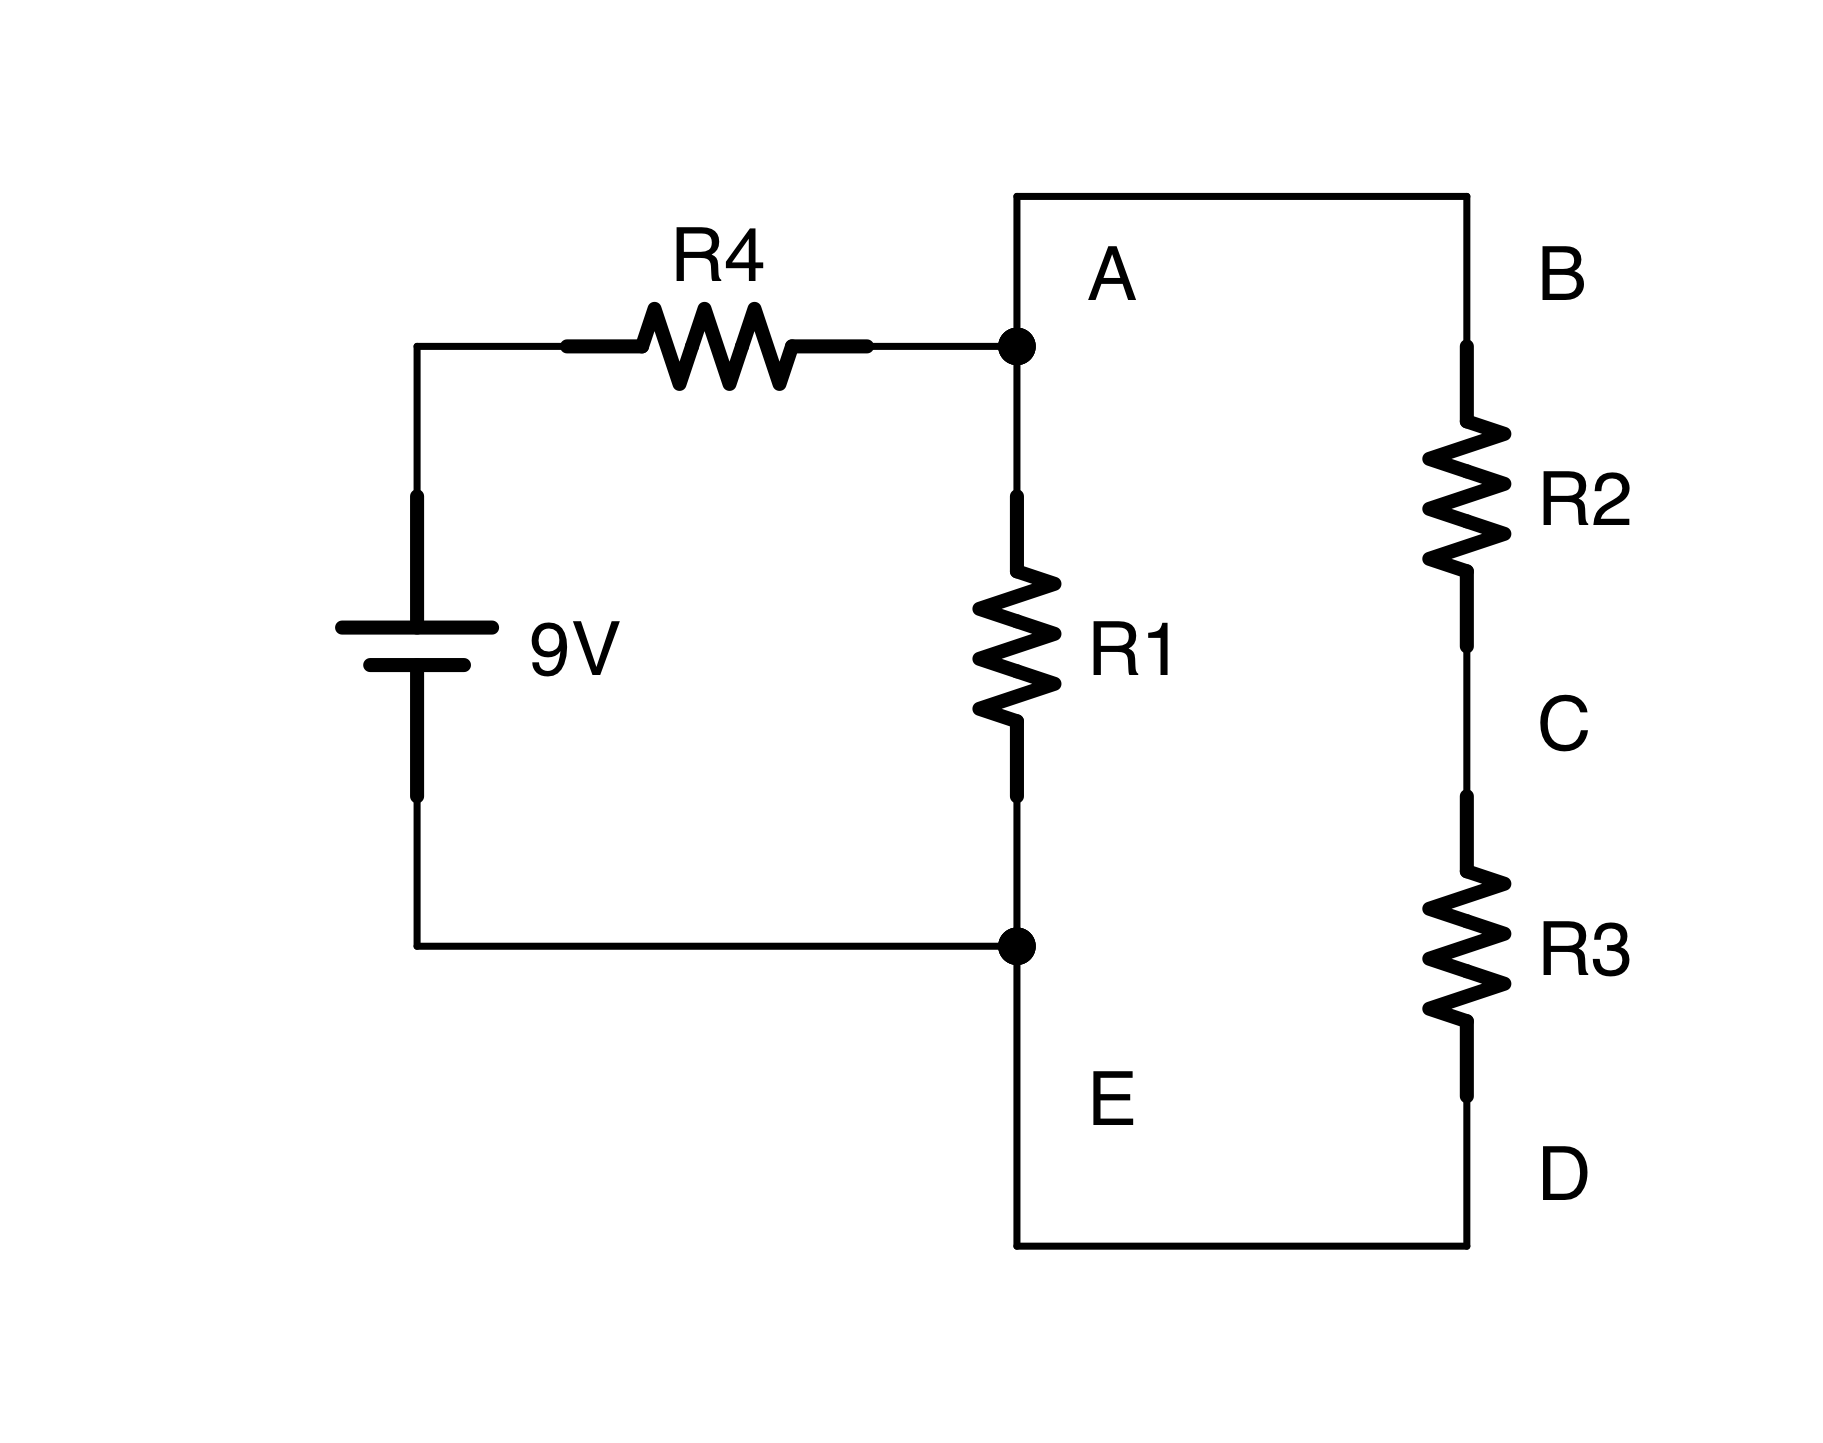
\includegraphics[scale=0.08]{VoltageDropProblem.png}
\item Optional - what resistor values would you need to have the circuit above run with $2\myamp$ total current?
\item The circuit below is a combination of series and parallel resistances.  Each resistor is labelled with its resistance value, given in ohms.  Find out how much current is flowing through each resistor, and how much each resistor drops the voltage.  \\ 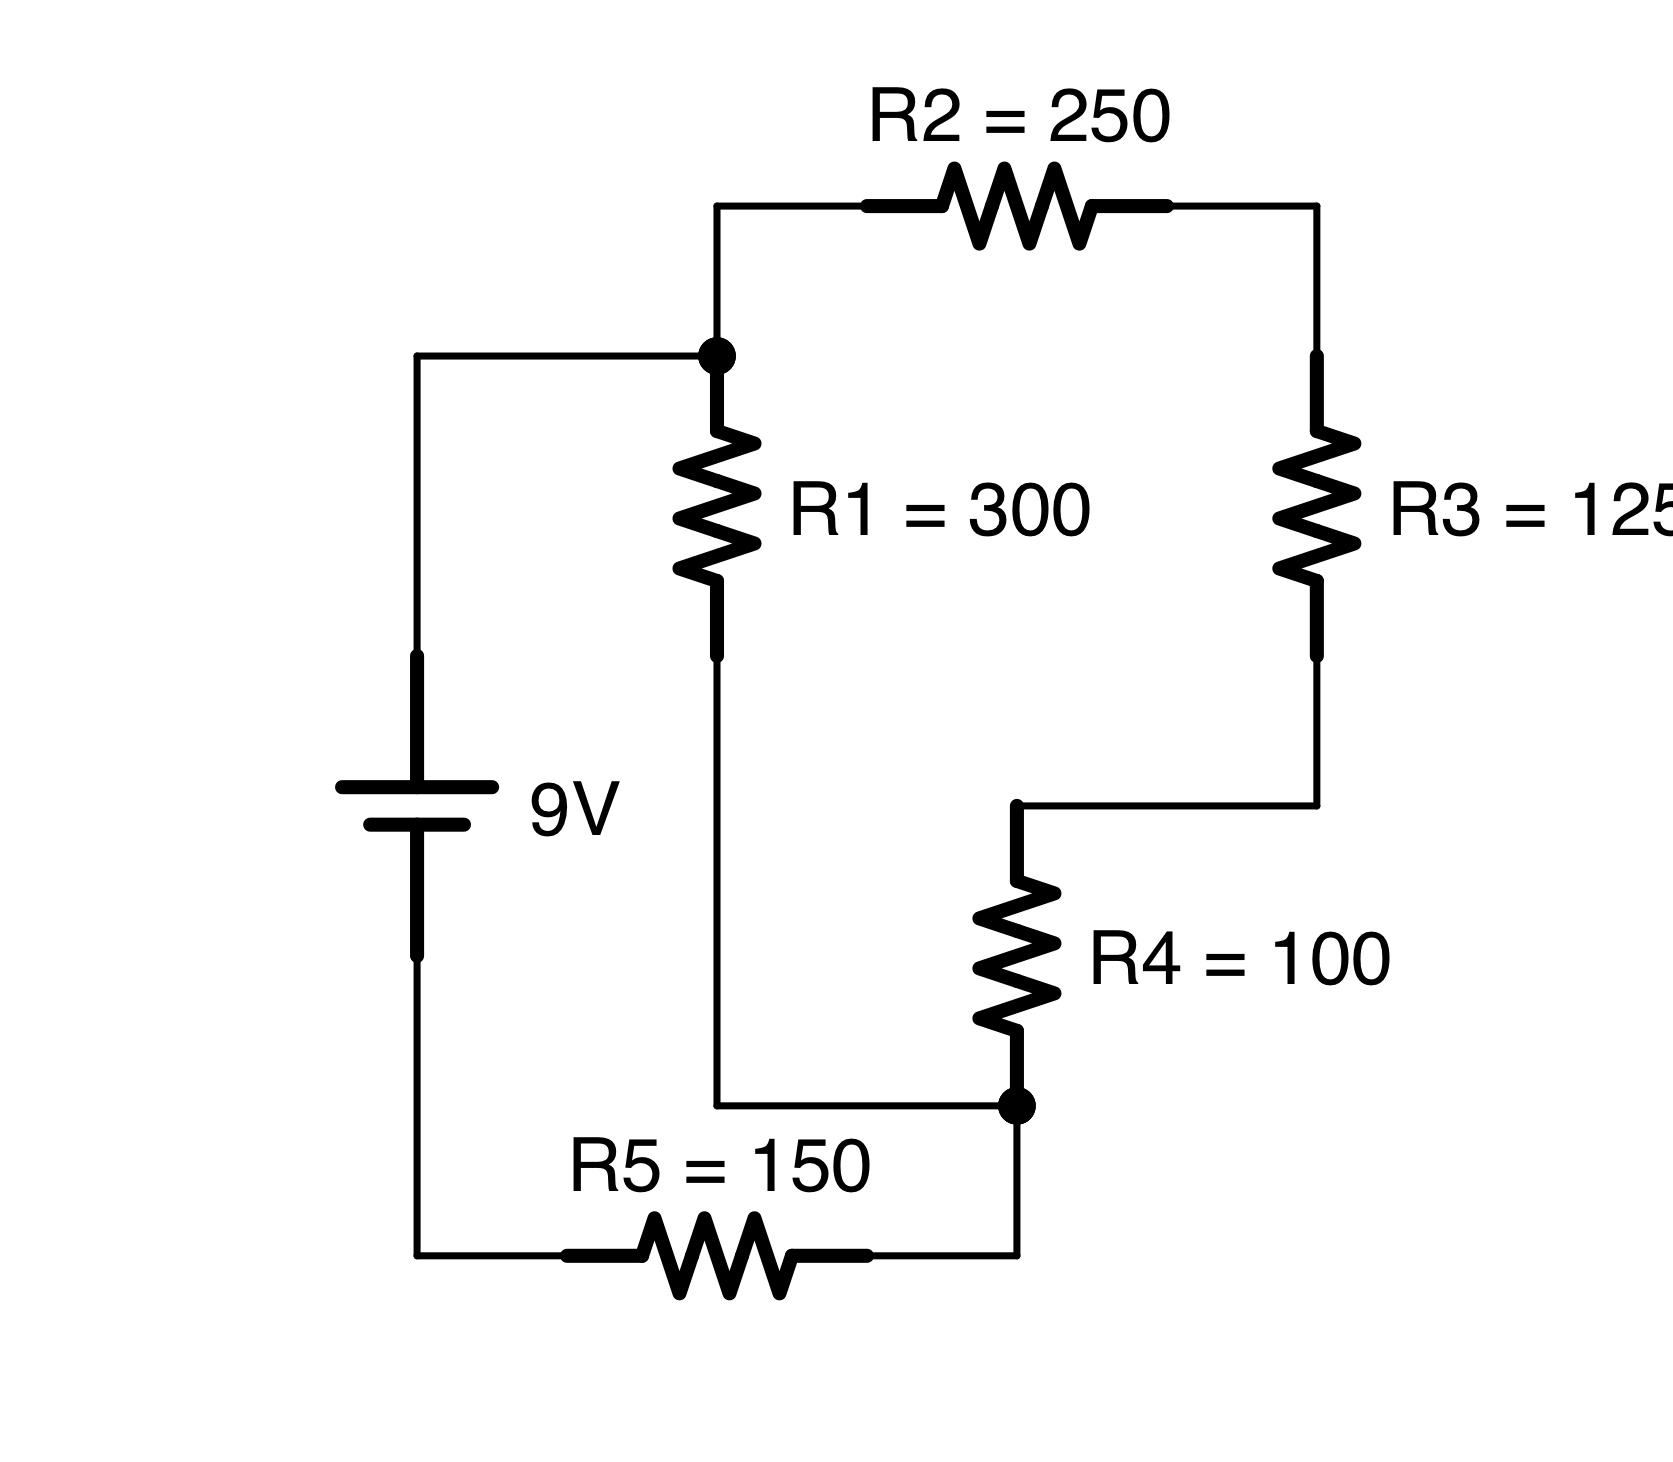
\includegraphics[scale=0.08]{ProblemCalculateCurrentAndVoltage.png}
\item Build the circuit in Figure~\ref{figParallelUsingBreadboard} on your own breadboard.  Measure the voltage drops across every component, and measure the amount of current flowing into the first series resistor.
\end{enumerate}
